\documentclass[sans,mathserif]{beamer}

\mode<presentation>
{
  \usetheme{Warsaw}
  % \usetheme{Madrid}
  % or ...

  %\setbeamercovered{transparent}
  % or whatever (possibly just delete it)
}

% \usepackage[czech]{babel}
\usepackage[utf8]{inputenc}

\usepackage{graphicx} % nezbytné pro standardní vkládání obrázků do dokumentu
\usepackage{multirow}

\usepackage{times}
\usepackage[T1]{fontenc}
% Or whatever. Note that the encoding and the font should match. If T1
% does not look nice, try deleting the line with the fontenc.

\newcommand{\xx}{\mathrm{\mathbf{x}}}
\newcommand{\yy}{\mathrm{\mathbf{y}}}
\newcommand{\ttheta}{\mathbf{\theta}}
\newcommand{\eell}{\boldsymbol\ell}
\newcommand{\uv}[1]{\quotedblbase #1\textquotedblleft}

\title[MGSO with Gaussian Processes for Black-Box Opt.
  \hspace{4em}\insertframenumber] % (optional, use only with long paper titles)
%   \hspace{2em}\insertframenumber/\inserttotalframenumber] % (optional, use only with long paper titles)
  {Model Guided Sampling Optimization with Gaussian Processes \\ for Expensive Black-Box Optimization}

\author[Luk\'{a}\v{s} Bajer, Viktor Charypar, Martin Hole\v{n}a]
{Luk\'{a}\v{s}~Bajer$^{1,2}$, Viktor Charypar$^3$ \and Martin Hole\v{n}a$^2$}
% - Give the names in the same order as the appear in the paper.
% - Use the \inst{?} command only if the authors have different
%   affiliation.

\institute[MFF UK, UI AVČR, FJFI ČVUT] % (optional, but mostly needed)
{
  $^1$Faculty of Mathematics and Physics, Charles University, and \\
  $^2$Institute of Computer Science, Czech Academy of Sciences \\
  $^3$Faculty of Nuclear Sciences, Czech Technical University
\vskip 1em
  Prague, Czech Republic
}
% - Use the \inst command only if there are several affiliations.
% - Keep it simple, no one is interested in your street address.

\date{GECCO, July 2013}
% \date[EvA 2008] % (optional, should be abbreviation of conference name)
% {AIL086 Evolutionary Algorithms 2}
% % - Either use conference name or its abbreviation.
% % - Not really informative to the audience, more for people (including
% %   yourself) who are reading the slides online

% \subject{Theoretical Computer Science}
% % This is only inserted into the PDF information catalog. Can be left
% % out. 

% If you have a file called "university-logo-filename.xxx", where xxx
% is a graphic format that can be processed by latex or pdflatex,
% resp., then you can add a logo as follows:

% \pgfdeclareimage[height=0.5cm]{mff-logo}{img/mff-logo}
% \logo{\pgfuseimage{mff-logo}}


% Delete this, if you do not want the table of contents to pop up at
% the beginning of each subsection:
\AtBeginSection[]
{
  \begin{frame}<beamer>{Contents}
  \tableofcontents[currentsection,currentsubsection]
  \end{frame}
}
% \AtBeginSubsection[]
% {
%   \begin{frame}<beamer>{Contents}
%   \tableofcontents[currentsection,currentsubsection]
%   \end{frame}
% }


% If you wish to uncover everything in a step-wise fashion, uncomment
% the following command: 

%\beamerdefaultoverlayspecification{<+->}


\begin{document}

\begin{frame}
  \titlepage
\end{frame}

\begin{frame}{Contents}
  \tableofcontents
  % You might wish to add the option [pausesections]
\end{frame}


% Structuring a talk is a difficult task and the following structure
% may not be suitable. Here are some rules that apply for this
% solution: 

% - Exactly two or three sections (other than the summary).
% - At *most* three subsections per section.
% - Talk about 30s to 2min per frame. So there should be between about
%   15 and 30 frames, all told.

% - A conference audience is likely to know very little of what you
%   are going to talk about. So *simplify*!
% - In a 20min talk, getting the main ideas across is hard
%   enough. Leave out details, even if it means being less precise than
%   you think necessary.
% - If you omit details that are vital to the proof/implementation,
%   just say so once. Everybody will be happy with that.

\section{Optimization of empirical functions}

\begin{frame}
  \frametitle{Optimization of expensive black-box functions}
  optimization of black-box functions
  \begin{figure}
  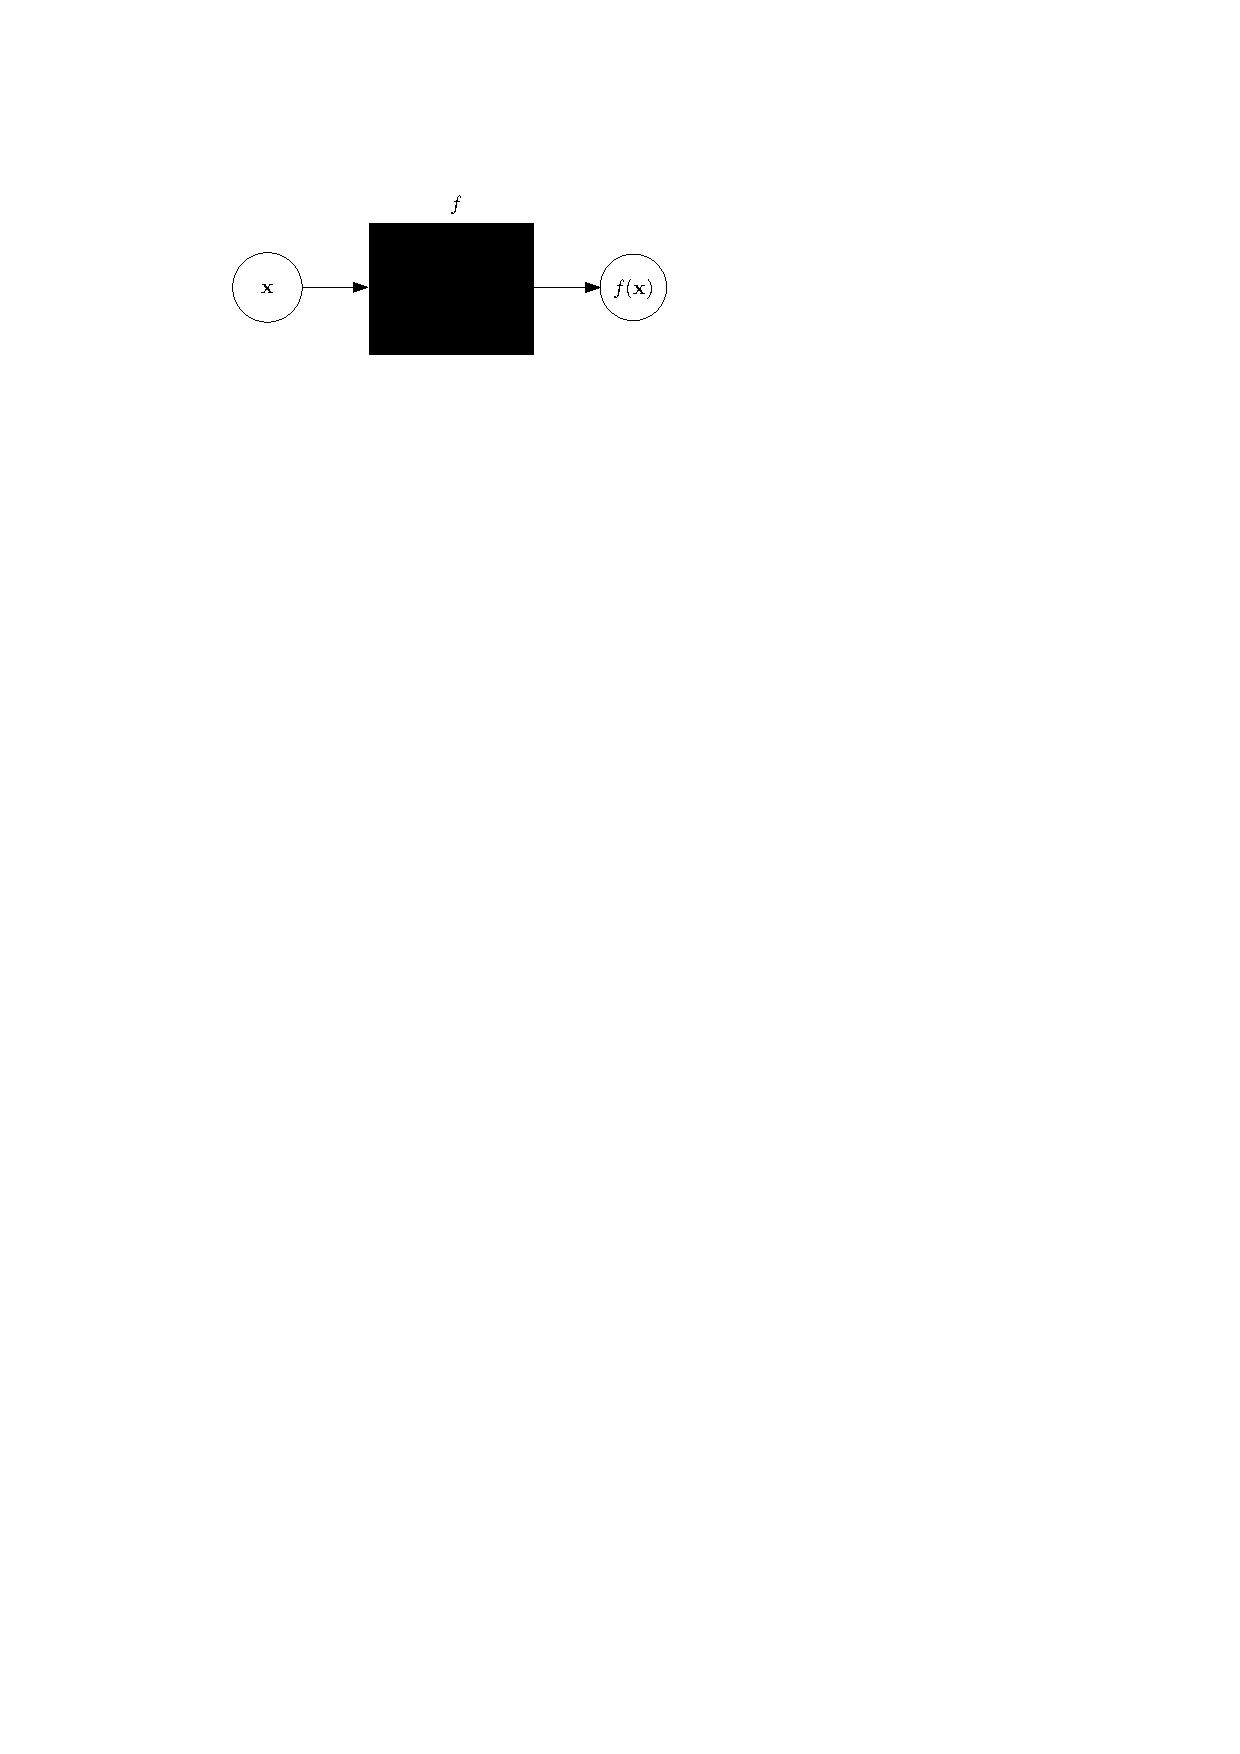
\includegraphics[width=0.6\linewidth]{img/black-box-function}
  % \caption{}
  \end{figure}
  \begin{itemize}
    \item continuous domain: $\xx \in \mathbb{R}^D$
    \item only evaluation of the function value, \\
      \alert{no derivatives} or gradients available
    \item evaluations are \alert{expensive} and/or time-demanding
    \item search cost $\sim$ the number of function evaluations
  \end{itemize}
\end{frame}

\end{document}

\begin{frame}
  \frametitle{}
  \begin{itemize}
    \item
  \end{itemize}
\end{frame}


